\section{Single-Task Feed-forward Neural Networks} \label{sec:singletaskNN}
% TODO: citations!
% TODO: check nn math 
% TODO: binary functions reppresentation theorem. 
\emph{Feed-forward neural networks} (FNN), also known as multilayer perceptron, are artificial neural network (ANN) that does not contains cycles. Despite many ANN models have failed the original attempts to mathematically reproduce the real structure of the brain they became an efficient model for pattern recognition. 

A feedforward neural network is described by a directed acyclic graph, $G =
(V,E)$, and a weight function over the edges, $w : E \to \mathbb R$ ($w(i, j) = 0$
for every $(i, j) \notin E$). Nodes of the graph correspond to neurons. Each
single neuron is modeled as a simple scalar function, $ \sigma : \mathbb R \to
\mathbb R$, this function is called \emph{activation function}. FNNs are usually
splitted in layers, that is the nodes in $V$ are decomposed in disjoint sets such
as for every layers $t \in T$ we have $V = \dot\cup_{t = 0}^T V_t$, $V_0$ and
$V_T$ are respectively called input and output layer, note that $|V_0| = d$ and
$|V_T| = n$ where $d$ is the dimensionality of the input space and $n$ the
dimensionality of the output space. Given the graph $G$, the map $w$ and the
activation function $\sigma$ the network is able to calculate the function
$f_{G,W,\sigma}$.  For every node $i \in V$ a value $v_i$ is associated and given $j
\in V \setminus V_0$ we define $w(j)$ and $v(j)$, for every $(i, j) \in E$, the
former is the vector containing all the weights $w(i, j)$ and the latter is the
vector whose component are the values $v_i$. Now the vector $f(x)$ is computed as
follow:
\begin{enumerate}
    \item $v_i = x_i$ for every node $i \in V_0$;
    \item $v_j = \sigma(w(j)^T v(j))$ for every node $j \in V \setminus V_0$;
    \item $f_k = v_k$, where k is the $k$th output node.
\end{enumerate}
In Figure~\ref{fig:neural_network_example} an example of neural network architecture is shown. \cite{ShwartzUnderstadningML, BishopML}
\begin{figure}[ht]
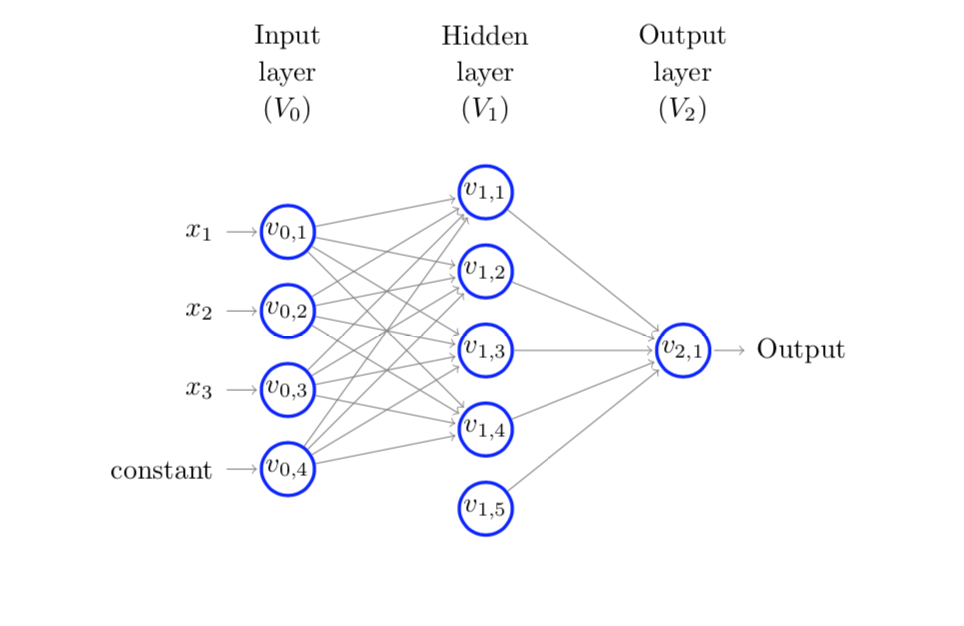
\includegraphics[width=\textwidth]{neural_network_example.png}
\caption{Deep Neural Network architecture example, it has a 3-dimensional input layer ($V_0$), one hidden layer ($V_1$) and a single neuron output layer ($V_2$) \cite{ShwartzUnderstadningML}.} 
\label{fig:neural_network_example}
\end{figure}

With the tuple $(G, \sigma)$, often called \emph{architecture of the network}, we can define the class of predictors: 
\[ \mathcal{F}_{G, \sigma} = \{ f_{G, \sigma, w} \mid w \textrm{ is a mapping from } E \textrm{ to } \mathbb R \} \]
From the standpoint of expressiveness of FNNs it is proved that with binary input $x \in \{-1, 1\}^d$, $mathrm{sign}$ as activation
function $\sigma$, a single hidden layer network is able to
implement every function $f: {-1, +1}^d \to {-1, +1}$. Note that the
binary constraint is just a useful simplification because, in
practical term, every real coordinates in a computer is represented
by a bit string of length $b$. That is, a single hidden layer is
enough to represent every Boolean functions. The downside is that
the number of neurons required must be exponential in the dimension
of the input space. Currently there is no mathematical proof on the
best network architecture, but there are some empirical evidence
that is better to place less neurons in many layers (deep learning)
rather than many neurons in a single layer. % TODO: citations

To train the weights of a feed-forward neural network is usually
used a gradient descent algorithm. The most common is called
Stochastic Gradient Descent (SGD), where, for every randomly sampled
example $x_t$ from the training set, the parameters $w(i, j)$ of the
network are update using the following rule:

\begin{equation} \label{eq:sgd} 
w(i, j) \leftarrow w(i, j) -  \eta_t \frac{\delta\ell_{x_t}(W)}{\delta w(i, j )}
\end{equation}

where $\ell_(.)$ is a convex loss function. SGD is not the only
gradient descent algorithm used, in the last year in order to
improve the convergence of the network many others were introduced,
such as mini-batch gradient descent, nesterov, adagrad
\cite{RuderGDOpt}. 

An algorithm called \emph{back-propagation} is used to compute the
gradient of the loss with respect of the weights in SGD. The
algorithm basically, using the chain rule of derivation, compute the
the gradient iterating backward layer by layer
\cite{HintonBackProp}.

%find best subsection title
\subsection{in our work}
% todo: explanation of our model 

\section{Multi-Task Neural Networks}\label{sec:MTLsection}
%TODO: soft and hard parameter sharing figures
Multi-Task learning (MTL) is became increasing popular in recent years. Usually, to optimizing the predictions of a given task, a single model is tuned and trained. Doing this good results can be achieved, but many information that might come from related task are lost. MTL methods take the signal from related tasks in consideration by sharing the representation between them. The typical settings is to learning multiple task simultaneously using a shared representation, what is learned by one task can be helpful for the others tasks and vice versa \cite{Caruana97}. There are many motivation behind MTL: from a biological point of view is inspired by the way human brain learn (the knowledge of tasks can help us learning other tasks), from a pure machine learning perspective, instead, can be view as a form of regularization where the inductive bias is introduced by the auxiliary tasks \cite{Ruder2017}. While in the past MTL was more used in non-neural models, more recently many deep learning works exploiting this approach were developed. In this context the two most used ways to perform multi-task learning are called \emph{soft parameters sharing} and \emph{hard parameter sharing}. In the former every tasks has his own set of parameters, the distance between this parameters is regularized in order to become similar and represent multiple tasks, noticeable example are \cite{duong-etal-2015-low} and \cite{yang2016trace}, in the latter instead a fixed number of hidden layers are shared between tasks and keeping several task specific output layers. In this works we have focused on hard-parameters sharing methods to implement our MTL network. Given $N$ the number of tasks, it is proved that hard-parameters sharing reduce the risk of over-fitting $N$ times compared to task-specific models \cite{baxter1997}.
\begin{figure}
\centering
\begin{subfigure}{.5\textwidth}
  \centering
  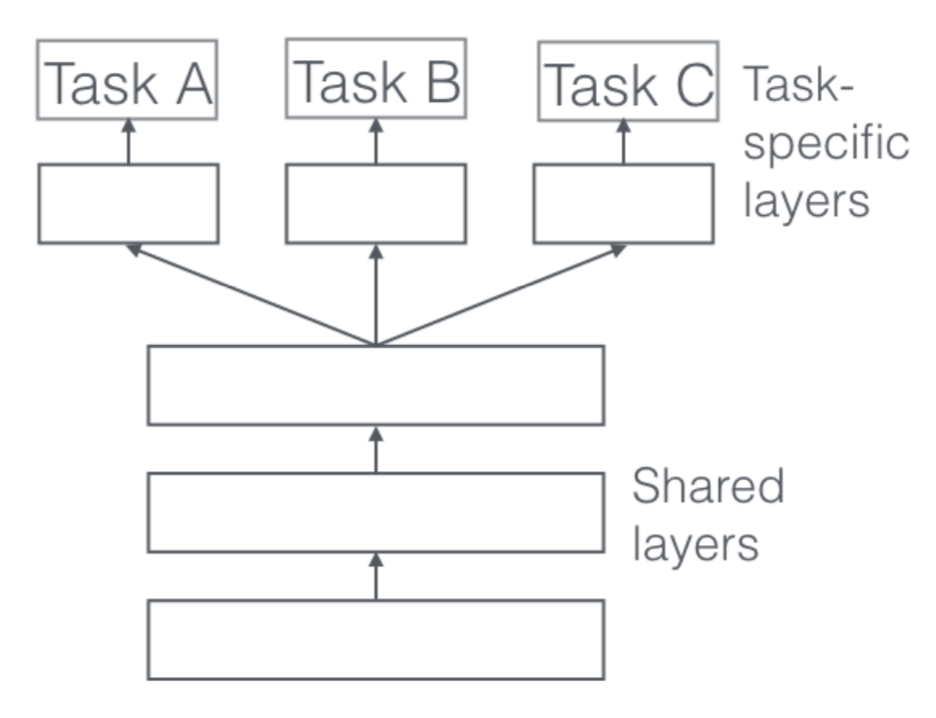
\includegraphics[width=.7\linewidth]{MTL_hard.png}
  \caption{A subfigure}
  \label{fig:sub1}
\end{subfigure}%
\begin{subfigure}{.5\textwidth}
  \centering
  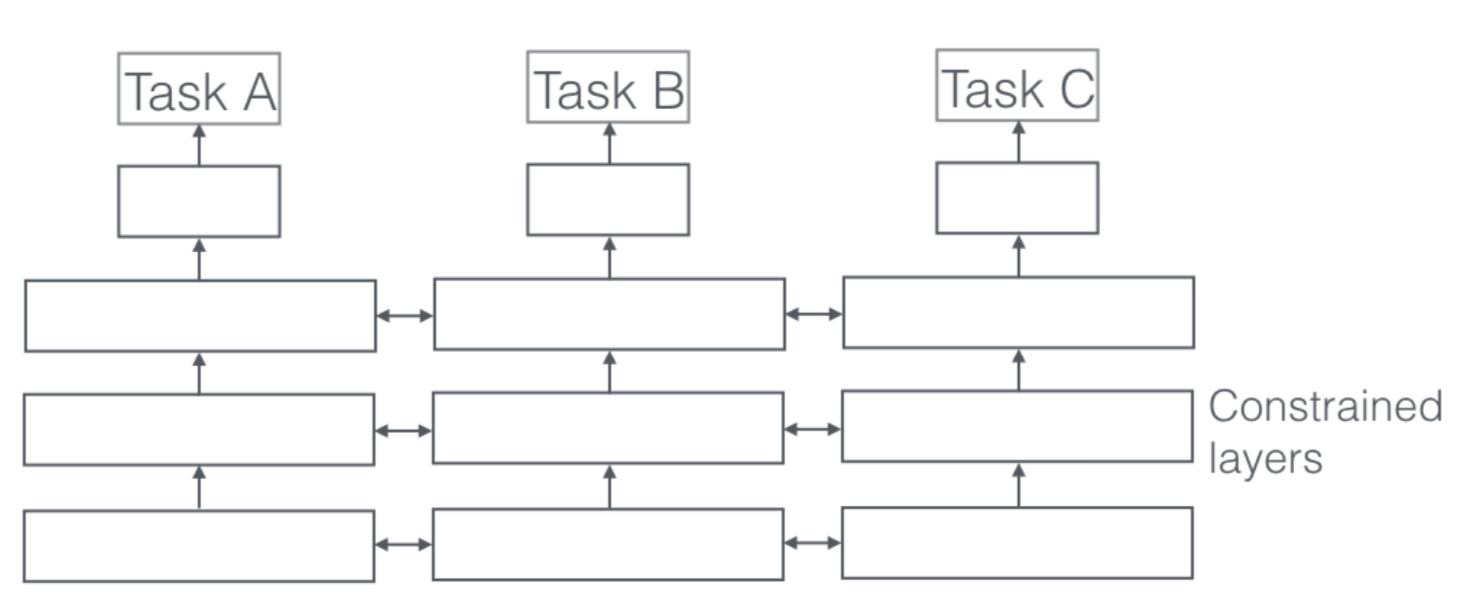
\includegraphics[width=1.2\linewidth]{MTL_soft}
  \caption{A subfigure}
  \label{fig:sub2}
\end{subfigure}
\caption{A figure with two subfigures}
\label{fig:test}
\end{figure}

\subsection{in our work}

\section{Gaussian Process for Hyper-parameters Tuning of the Models}
% todo: integrate
% todo: read again
% todo: images
% todo: fix mathematical formalization (???)
In Section~\ref{sec:singletaskNN} and Section~\ref{sec:MTLsection} we
described single-task and multi-task approach for training neural
networks from a theoretical point of view. In practice, due to the
growing complexity of deep learning models, working with neural networks
involves a proper choice of many hyper-parameters, such as the shape of
the network architecture, the learning rate, or the regularizer weight
decay. Over the years many hyper-parameters optimization algorithms were
proposed, grid and random search \cite{BergstraB12} are two important
examples. A more sophisticated model is exploiting bayesian optimization
and use it to choose the best hyper-parameters for a given model
\cite{SnoekGP}. In general, the aim of optimizers is to minimize (or
maximize) a scoring function respect its hyper-parameters, given
$\mathcal{X}$ the set of hyper-parameters and $f(x)$ the scoring function
(i.e., auprc, auroc, rmse, binary loss etc.) we have: 
\[ 
x^* =  \argmin_{x \in \mathcal{X}} f(x) 
\]
the main difference between bayesian optimization respect the more
traditional approaches is that, bayesian optimization, choose the next
hyper-parameters set in an informed way keeping track of past evaluations
that use to build a probabilistic model called \emph{surrogate function}, often build using a Gaussian process. That is, in every
iteration the surrogate function is updated selecting, using a
\emph{selection function} such as Expected Improvement (EI), and
evaluating a new set of hyper-parameters. On one hand bayesian methods
take more time choosing the next set of hyper-parameters, on the other
hand they make few iterations compared to grid and random search. 
Recently Keras developer have released a new hyper parameter optimizer
open-source library called Keras-tuner \footnote{Available on GitHub:
\url{https://github.com/keras-team/keras-tuner}}
\cite{omalley2019kerastuner}, it contains, among many others, an
implementation of bayesian optimization\footnote{Documentation available
at: \url{https://keras-team.github.io/keras-tuner/documentation/tuners/}}.

\section{Evaluation Metrics}
In this section the principal evaluation metrics used in this work are described. 
% todo: loss funtion better in another section?
In Section~\ref{sec:singletaskNN} we described Stochastic Gradient Descend algorithm, in Equation~\ref{eq:sgd} we seen that, in order to update the parameters of the network, we need to calculate the derivative of a convex loss function $\ell(.)$ respect the weights. In this work, in order to train both single and multi task neural networks, we utilized a well-known loss function, often used in binary classification, called \emph{binary cross-entropy}. Given $t \in \{0, 1\}$, the true binary label of a sample, and $s \in [0, 1]$, the probability score given by a predictor, we define binary cross-entropy as:
\begin{equation}
    \ell(t, s) = -tlog(s) - (1 - t)log(1 - s)
\end{equation}

In order to evaluate the performance of the models, many metrics can be used. Despite its simplicity, one of the most popular is \emph{Accuracy} defined as the proportion of the correct respect the total number of sample
\begin{equation}
    \textrm{accuracy} = \frac{\#\{\textrm{correct samples}\}}{\#\{\textrm{total samples}\}}
\end{equation}
It is easy to notice that the main drawback of accuracy is that, with unbalanced dataset, we can achieve a misleading higher values. Fortunately, during the years, more stable performance evaluation metrics were introduced in order to overcome accuracy disadvantages. Before describing this new metrics, in the contest of binary classification, we must introduce four classification terms: 
\begin{itemize}
\item \emph{True Positive} (TP): samples classified as positive where also the actual value is positive;
\item \emph{False Positive} (FP): samples classified as positive where the actual values is negative;
\item \emph{True Negative} (TN): samples classified as negative where also the actual values is negative;
\item \emph{False Negative} (FN): samples classified as negative where the actual values is positive.
\end{itemize}
Of course, the aim of a good model is to have a very high true positive and true negative. From this point of view, to evaluate the goodness of a model we can use some metrics called \emph{precision} and \emph{recall}. Precision evaluate the ability of a model to correctly classify relevant results
\begin{equation}
    \textrm{precision} = \frac{\textrm{TP}}{\textrm{TP}+\textrm{FP}}
\end{equation}
recall, instead, is the percentage of total relevant results correctly classified by your algorithm 
\begin{equation}
    \textrm{recall} = \frac{\textrm{TP}}{\textrm{TP}+\textrm{FN}}
\end{equation}
this two metrics are often putted together using harmonic mean, the resulting metric is called \emph{F1-score}:
\begin{equation}
    \textrm{F1-score} = 2 \cdot \frac{\textrm{precision} \cdot \textrm{recall}}{\textrm{precision}+\textrm{recall}}
\end{equation}
Finally, we describe the two main metrics used to evaluate the performance of the models used in this work: \emph{Area Under the Receiver Operating Characteristics} (AUROC) and \emph{Area Under the Precision-Recall Curve} (AUPRC). 
The AUROC is computed plotting the ROC curve with Recall on y-axis against False Positive Rate (FPS) on x-axis and calculating the area under it.  Similarly, AUPRC is computed plotting precision on y-axis against recall on x-axis and calculating the area under it. Since both precision and recall does not consider true negative sample, AUPRC is used when having good performance on negative example are not extremely important. 